\documentclass[a4paper,11pt]{article}
\usepackage{geometry}
\geometry{
    margin=0.3in,    % Adjust margins for proper spacing
    bottom=0.25in,   % Allow space for footer
    footskip=0.1in   % Space for the footer
}
\usepackage{fancyhdr}
\usepackage{titlesec}
\usepackage{graphicx}
\usepackage{amsmath}
\usepackage{hyperref}
\usepackage{float}
\usepackage{caption}
\usepackage{booktabs}
\usepackage{cleveref}
\usepackage{pgfplots}
\usepackage{placeins} % Add this to your preamble
\pgfplotsset{compat=1.17}

% Custom title setup
\newcommand{\customtitle}{
    \begin{center}
        \textbf{\LARGE {Module ENGI2221: Mechanics, 2024/25}} \\[0.5cm]
        \textbf{\Large Jiaxi Wang}
    \end{center}
}

\hypersetup{
    colorlinks=true,
    linkcolor=blue,
    filecolor=magenta,
    urlcolor=cyan,
    pdftitle={Stress Concentrations in Solid Mechanics},
    pdfauthor={Your Full Name},
    bookmarksopen=true,
    bookmarksnumbered=true
}

% Header and Footer Setup
\pagestyle{fancy}
\fancyhf{} % Clear all header and footer fields

 % Define footers
\fancyfoot[C]{\textbf{Page~\thepage~of~8}}
% Default footer
\fancyfoot[R]{\textbf{continued}}

% Redefine footer for the last page only
\AtEndDocument{%
  \fancyfoot[R]{}
}


% Remove header and footer rules
\renewcommand{\headrulewidth}{0pt}
\renewcommand{\footrulewidth}{0pt}
 

% Section Formatting
\titleformat{\section}[block]{\bfseries\Large}{\thesection.}{1em}{}
\titleformat{\subsection}[block]{\bfseries\large}{\thesubsection.}{1em}{}

% Paragraph spacing
\setlength{\parindent}{0pt} % No paragraph indentation
\setlength{\parskip}{4pt}   % Spacing between paragraphs

 


\begin{document}



% Title block at the top
\customtitle
% Page 1: Summary and Introduction

 
{\small
\tableofcontents
}


% List of Figures
\listoffigures % Generates the list of figures
 \vspace{-10pt}
\vspace{-10pt}
\section*{Summary}
\vspace{-10pt}
This report investigates stress concentration in structural elements, with a focus on aerospace applications. Stress concentrations, caused by geometric discontinuities such as elliptical apertures in pressurized thin-walled cylinders and circular holes in plates, significantly affect the durability and safety of aerospace components. Theoretical analysis explores the relationship between tangential stress ($\sigma_t$) and stress concentration factors ($K_t$), highlighting how material yield strength limits structural performance. Numerical simulations using \textit{Concept Analyst} software \cite{conceptanalyst2024} evaluate how variations in geometric parameters, such as aperture size and spacing, influence $K_t$ in plates. The findings underscore the importance of managing stress concentrations to improve the durability, fatigue resistance, and reliability of aerospace structures. Specifically, this research aids in optimising designs for pressurized aircraft fuselages, contributing to safety under cyclic loading. The report also recommends advanced materials, such as titanium alloys and CFRP, for reinforcing high-stress regions, enhancing both structural integrity and weight efficiency in aircraft like the Airbus A350.
\vspace{-15pt}
\section{Introduction: Stress Concentrations in Aerospace Structures}
\vspace{-15pt}
Stress concentrations, arising from geometric discontinuities such as holes, notches, and cutouts, determining the structural integrity and safety of aerospace components. These stress risers are significant under cyclic loading conditions, where repeated pressurisation and aerodynamic forces in fuselage and wing structures can lead to fatigue crack initiation and propagation. Rapid decompression of a Southwest Airlines Boeing 737-700 \cite{ntsb2019} and Aloha Airlines Flight 243 \cite{ntsb1989}, underscore the devastating consequences of insufficiently addressing these localised stress peaks. Fuselage windows, access ports, and fastener holes, introduce unavoidable stress concentrations, necessitating designs that balance structural resilience with functionality. Elliptical windows are favored over rectangular counterparts due to their reduced stress concentration factors ($K_t$), which typically range from 2 to 10 in aerospace-grade materials like aluminum alloys and composites under tension, compression, or shear loading \cite{pilkey2020}. These stress levels are compounded by high-pressure loads and frequent operational cycles common in aerospace environments, often exceeding 35,000 pressurization cycles during an aircraft’s lifetime\cite{megson2016}.  By examining geometric spacing, orientation, and diameter-to-width ratios ($d/W$) using Concept Analyst, the study aims to propose optimized mitigation strategies for stress reduction. The approach aligns with industry standards, including FAA AC 25.571-1D \cite{faa_ac_25_571_1d}, which provides guidelines for damage tolerance and fatigue evaluation in critical structures. 
 
\vspace{-15pt}
\section{Theory:Stress Concentrations Around Elliptical Openings}
\vspace{-15pt}
 

For thin-walled cylinders subjected to internal pressure (\(p\)), the principal stresses—hoop stress (\(\sigma_{\text{hoop}}\)) and axial stress (\(\sigma_{\text{axial}}\))—are expressed as:
\begin{equation}
\sigma_{\text{hoop}} = \frac{pR}{t}, \quad \sigma_{\text{axial}} = \frac{pR}{2t} \cite{benham1996}.
\label{eq:thin_wall}
\end{equation}
Here, \(R\) is the cylinder’s radius, and \(t\) is the wall thickness. The factor of 2 comes from the distribution of force across the entire cross-sectional area of the cylindrical wall. It assumes a thin-wall condition (\(R/t \gg 1\)), which is valid for most aircraft fuselages \cite{young2011}. The hoop stress, being twice the axial stress, dominates the structural behavior.

The total tangential stress (\(\sigma_{\beta\beta, \text{total}}\)) around the cylinder includes contributions from both the hoop and axial stresses:
\begin{equation}
\sigma_{\beta\beta, \text{total}} = \sigma_{\beta\beta, \text{hoop}} + \sigma_{\beta\beta, \text{axial}}\cite{savin1961}
\end{equation}


 \vspace{-15pt}
\begin{minipage}{0.45\textwidth}
\begin{equation}
\sigma_{\beta\beta, \text{hoop}} = \sigma_{\theta\theta} \cdot \frac{\sinh(2\alpha_0) - 1 + e^{2\alpha_0} \cos(2\beta)}{\cosh(2\alpha_0) - \cos(2\beta)}
\end{equation}
\vspace{-15pt}
\end{minipage}%
\hfill
\begin{minipage}{0.45\textwidth}
\begin{equation}
\sigma_{\beta\beta, \text{axial}} = \sigma_{zz} \cdot \frac{\sinh(2\alpha_0) + 1 - e^{2\alpha_0} \cos(2\beta)}{\cosh(2\alpha_0) - \cos(2\beta)}
\end{equation}
\vspace{-15pt}
\end{minipage}

 


 

Geometric discontinuities, such as elliptical apertures, significantly amplify local stresses. Using Inglis’ solution \cite{inglis1913}, the tangential stress (\(\sigma_t\)) around the rim of an elliptical opening subjected to far-field stress (\(\sigma_\infty\)) is given by:
\begin{equation}
\sigma_e = S \left( \frac{\sinh(2\alpha_0) - 1 + e^{2\alpha_0} \cos(2\beta)}{\cosh(2\alpha_0) - \cos(2\beta)} \right) 
+ S \left( \frac{\sinh(2\alpha_0) + 1 - e^{2\alpha_0} \cos(2\beta)}{\cosh(2\alpha_0) - \cos(2\beta)} \right) \cite{ghali2009}.
\label{eq:tangential_stress}
\end{equation}

 \(a\) and \(b\) are the semi-major and semi-minor axes of the ellipse, \(\alpha_0 = \tanh^{-1}(b/a)\), quantifies the ellipse’s aspect ratio.\(\beta\) represents the angular position along the elliptical rim. The stress concentration factor (\(K_t\)) characterizes the amplification of stress at the edge of the opening:
  
\begin{equation}
K_t = \frac{\sigma_{\text{max}}}{\sigma_{\text{nom}}}\cite{peterson1974}
\label{eq:stress concentration factor}
\end{equation}
 \vspace{-10pt}

In this context, \(\sigma_{\text{max}}\) is the peak stress at the edge of the opening, and \(\sigma_{\text{nom}}\) is the nominal stress in the absence of the aperture. The elliptical geometry magnifies stresses along the major axis, making it a critical design consideration.



     
 
 

  



   
 \vspace{-10pt}


\section{Theoretical Analysis of Fuselage Window Stresses}
 \vspace{-10pt}

 \vspace{-10pt}
\begin{table}[h!]
\centering
\begin{tabular}{|l|l|}
\hline
\textbf{Parameter}                & \textbf{Value}                    \\ \hline
Fuselage diameter ($D$)           & $5.96$ m                          \\ \hline
Fuselage radius ($R$)             & $\frac{D}{2} = 2.98$ m            \\ \hline
Wall thickness ($t$)              & $0.002$ m                         \\ \hline
Elliptical window semi-major axis ($a$) & $0.1$ m                          \\ \hline
Elliptical window semi-minor axis ($b$) & $0.09$ m                         \\ \hline
Internal pressure differential ($p$)   & $61$ kPa $= 0.061$ MPa           \\ \hline
\end{tabular}
\caption{Initial Parameters for the Airbus A350-900 Fuselage Model}
\label{tab:initial_parameters}
\end{table}
 \vspace{-20pt}
 
 

\subsection{Base Fuselage Stresses,Stress Concentration Factor and Maximum Stress}
 \vspace{-10pt}
Using the thin-walled cylinder equations, as defined in 
Equation~\ref{eq:thin_wall}:

\noindent
\begin{minipage}{0.45\textwidth}
\begin{equation}
\sigma_{\text{hoop}} = \frac{(0.061)(2.98)}{0.002} = 90.89 \, \text{MPa}
\end{equation}
\end{minipage}%
\hfill
\begin{minipage}{0.45\textwidth}
\begin{equation}
\sigma_{\text{axial}} = \frac{(0.061)(2.98)}{2(0.002)} = 45.445 \, \text{MPa}
\end{equation}
\end{minipage}
 
 
The tangential stress around the rim of an elliptical hole under far-field stress \( S \) is shown in Equation~\ref{eq:tangential_stress}, The parameter \( \alpha_0 \) is computed as:
\begin{equation}
\tanh \alpha_0 = \frac{b}{a} \implies \alpha_0 = \tanh^{-1}\left(\frac{b}{a}\right) = \tanh^{-1}\left(\frac{0.09}{0.1}\right) = \tanh^{-1}(0.9) \approx 1.472
\end{equation}
 


 
 
 
\begin{figure}[ht]
 
    \centering
 
        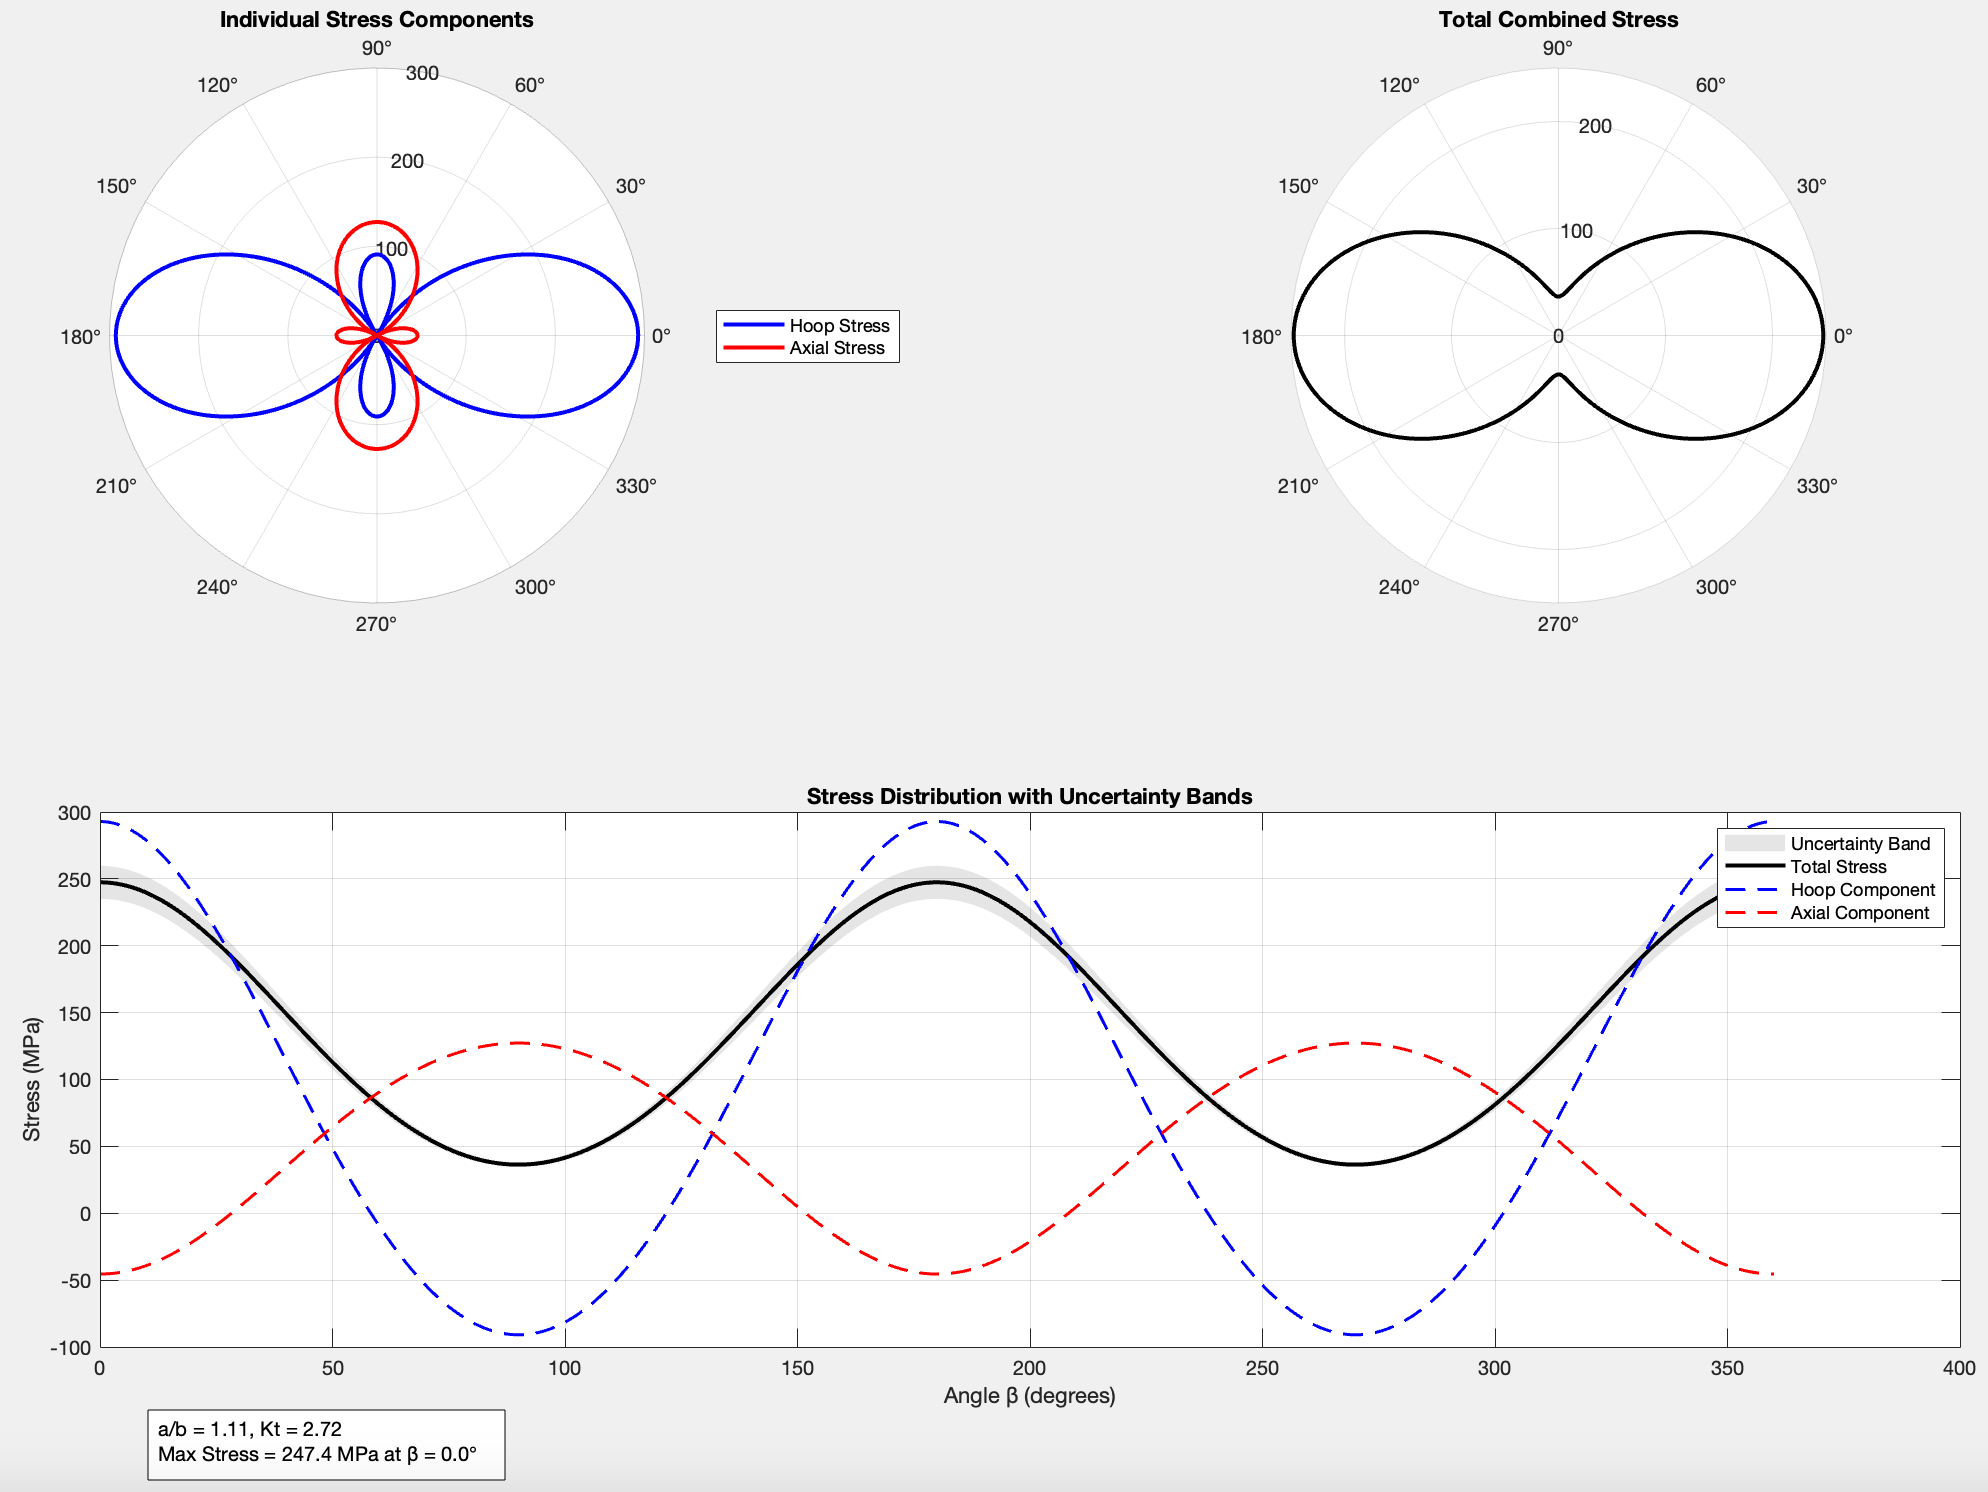
\includegraphics[width=\textwidth]{Screenshot 2025-01-03 at 22.49.55.png}
        \caption{Tangential Stress Distribution (Cartesian and Polar Plot)}
        \label{fig:stress_distribution_polar}
 
\end{figure}




 

\begin{table}[h!]
\centering
\renewcommand{\arraystretch}{1.3}
\begin{tabular}{|c|c|}
\hline
\textbf{Parameter}                      & \textbf{Value}                              \\ \hline
\textbf{Analysis for a/b}               & 1.11                                       \\ \hline
\textbf{Base Hoop Stress (\( \sigma_{\text{hoop}} \))} & 90.89 MPa                                 \\ \hline
\textbf{Base Axial Stress (\( \sigma_{\text{axial}} \))} & 45.45 MPa                                 \\ \hline
\textbf{Maximum Stress (\( \sigma_{\max} \))}        & 247.42 MPa at \( \beta = 0^\circ, 180^\circ \)     \\ \hline
\textbf{Minimum Stress (\( \sigma_{\min} \))}        & 36.36 MPa at \( \beta = 90^\circ, 270^\circ \)   \\ \hline
\textbf{Stress Concentration Factor\cite{peterson1974} (\( K_t \))} 
    & \( K_t = \frac{\sigma_{\text{max}}}{\sigma_{\text{nom}}} = 2.72 \) \\ \hline
\end{tabular}
\caption{Stress Analysis Results for an Elliptical Window with a/b = 1.11}
\label{tab:analysis_results}
\vspace{-15pt}
\end{table}
 
 
 \section{Stress Distribution Around an Elliptical Window in a Pressurized Fuselage}
 
The stress distribution around an elliptical window in a pressurised fuselage reflects the interaction between the baseline biaxial stress field and the localized modifications induced by the geometric discontinuity. The hoop stress (\(\sigma_{\text{hoop}} = \frac{pR}{t}\)) and axial stress (\(\sigma_{\text{axial}} = \frac{pR}{2t}\)) create the primary stress field, while the elliptical opening amplifies local stresses according to its geometry (\(a/b\)) and angular position (\(\beta\)). Maximum stresses occur at \(\beta = 0^\circ\) and \(180^\circ\) due to alignment with the hoop stress and the curvature of the major axis, with \(\sigma_{\text{max}} = 247.42 \, \text{MPa}\). Minimum stresses at \(\beta = 90^\circ\) and \(270^\circ\) reduce to \(\sigma_{\text{min}} = 36.36 \, \text{MPa}\). 
The sharp curvature around elliptical windows amplifies stress concentrations, disrupting the primary hoop stress, which is already twice as large as the axial stress due to pressurization. The alignment of the major axis with the hoop direction creates stress hotspots at the window's endpoints. Stress amplification arises from strain compatibility, boundary curvature, and membrane effects, making reinforcement with materials like CFRP or titanium alloys essential.  


 \subsection{Comparison of properties of various aerospace materials for fuselage design}
\begin{table}[h!]


\renewcommand{\arraystretch}{0.85}
\setlength{\tabcolsep}{14pt}
\makebox[\textwidth][c]{%
\begin{tabular}{|p{3.5cm}|p{2cm}|p{1.5cm}|p{9cm}|}
\hline
\textbf{Materials for  fuselages}& \textbf{Yield Strength (\( \text{MPa} \))}& \textbf{Safety Factor (\( SF \))} & \textbf{Analysis:} 
fatigue loading , repeated pressurization cycles, environmental degradation , corrosion , UV exposure, stemming from manufacturing tolerances\\ \hline
Aluminum 7075-T6           & 503 \cite{matweb7075} & \( 2.03\)& Meets aerospace safety standards (\( SF > 1.5 \));strength and reliability, feasible option for non-critical regions\\ \hline
Aluminum 2024-T3           & 345  \cite{aircraftaluminium}                                                       & \( 1.39 \)& Safety factor too low compare to ISO standard \cite{nasa2015}; unsuitable for high-stress areas.                                          \\ \hline
CFRP (Carbon Fiber)        & 800  \cite{{rosap2024}}                                              & \( 3.23 \)& Excellent safety margin, fatigue resistance, and strength-to-weight ratio; ideal for primary structures. Resistance to fatigue and crack propagation\\ \hline
Titanium Alloy (Ti-6Al-4V) & 880 \cite{carpenterTi64}                                                         & \( 3.56 \)& Significant safety margin; critical regions like window frames and egdes due to excellent fatigue properties.\\ \hline
\end{tabular}%
}
\caption{Comparison of Aerospace Materials for Fuselage Design}
\label{tab:material_comparison}
\end{table}


 

In high-stress areas like window frames, titanium reinforcements or hybrid CFRP-titanium structures are recommended. While aluminum alloys such as 2024-T3 are inadequate for these regions, 7075-T6 offers only marginal safety margins. In contrast, CFRP and titanium alloys provide superior safety factors, making them ideal for modern fuselage designs. For instance, the A350 utilizes CFRP \cite{airbus_a350} in the primary structure and titanium reinforcements in high-stress zones to optimize both strength and weight efficiency. CFRP offers tailored strength distribution and excellent fatigue resistance but requires careful attention to interlaminar shear strength\cite{ecrc_template}, especially near window edges, to prevent delamination. Fiber orientation must be optimized, and protective coatings are essential to mitigate environmental aging. Titanium alloys (Ti-6Al-4V) excel in fatigue performance and crack propagation resistance, and they integrate well with CFRP in hybrid structures. However, careful design is necessary to prevent galvanic corrosion at metal-composite interfaces and manage differential thermal expansion. For optimal performance, CFRP should be used in the primary fuselage structure with a tailored fiber architecture to handle biaxial loading, and health monitoring systems should be integrated for long-term reliability. In high-stress regions, Ti-6Al-4V reinforcements are recommended, and hybrid CFRP-titanium solutions offer an ideal combination of strength, fatigue resistance, and weight efficiency.



\begin{table}[ht]

\subsection{Effects on the stress distributions of multiple windows }

\centering
\renewcommand{\arraystretch}{1}
\setlength{\tabcolsep}{1pt}
\makebox[\textwidth][!]{%
\begin{tabular}{|p{3cm}|p{8cm}|p{8cm}|}
\hline
\textbf{Aspect}                  & \textbf{Key Considerations}                                                                                      & \textbf{Mitigation Strategies}                                                                             \\ \hline
Stress Field    & Overlapping stress fields between closely spaced windows amplify peak stresses, creating alternating high/low stress zones. & Reinforce regions between windows and analyze for periodic stress distributions during design.            \\ \hline
Load Path          & Stresses flow around openings, creating localized high-stress paths. Inter-window regions bear higher stresses and buckling.& Add reinforcements like doublers, use load-sharing design elements, and analyse combined operational loads.\\ \hline
Edge Effects                     & End windows in rows experience higher stresses due to less redundancy; transition regions have complex stress patterns.      & Increase structural redundancy at row ends and enhance design around transition regions.                   \\ \hline
Geometric Effects                & Close spacing increases stress interaction; wide spacing reduces stress wastes  space.& Optimize spacing to balance stress reduction and structural efficiency.                                    \\ \hline
Global  Impact& Multiple windows reduce fuselage stiffness, increase deformation, and affect vibration modes and dynamic response.           & Assess global deformation and dynamic response; stiffen critical areas to maintain structural performance. \\ \hline
Fatigue         & Cyclic loading induces fatigue in window regions, accelerating crack initiation.& Employ tear straps, fatigue-resistant materials, and rigorous fatigue testing.                            \\ \hline
 Implications Strategy& Overlapping Stress Fields, Load Redistribution,Reduced Structural Stiffness& reinforcement frames, thickened skin sections, and strict manufacturing tolerances.\\ \hline
\end{tabular}%
}
\caption{Key Structural Considerations and Mitigation Strategies for Window Design}


\label{tab:structural_considerations}
\end{table}
 

The analysis of multiple aircraft windows presents significant design challenges, as detailed in Table~\ref{tab:structural_considerations}. Overlapping stress fields between adjacent windows increase stress amplification compared to single windows\cite{pilkey2020peterson}. Modern designs, such as the Airbus A350, utilise composite reinforcement frames and optimized spacing, achieving lower stress concentrations than traditional aluminum structures\cite{kassapoglou2013design}.  

 
\begin{figure}[H] % [H] places the figure exactly where it appears in the code
 
\subsection{Key assumption and validity}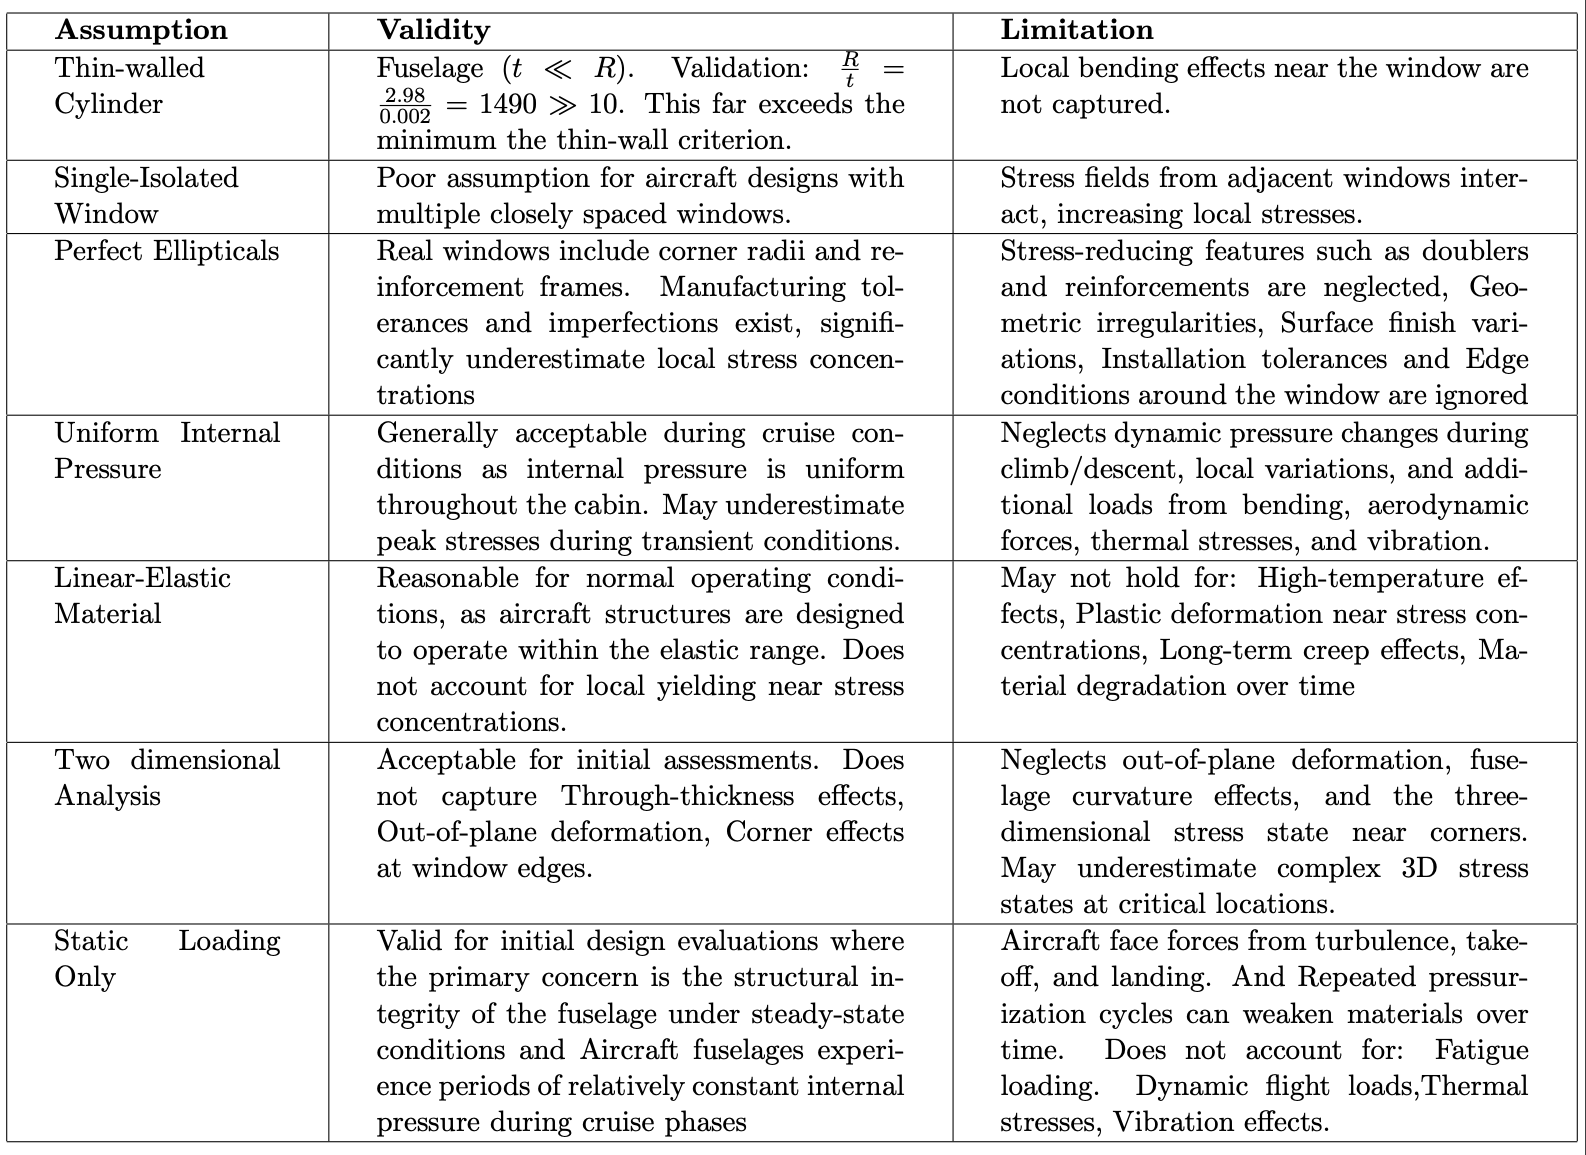
\includegraphics[width=0.99\textwidth]{table1.png} % Replace with your image file name (without extension)
    \caption{assumption and validity of stress analysis }


\label{tab:assumption and validity}
\end{figure} 


 
 
\vspace{-20pt} % Reduce space before figure

\section{Computational simulations :Variation of Kt with r/d,\(\theta\) and size of the plate}

\vspace{-10pt} % Reduce space before figure
The stress concentration analysis was performed using Concept Analyst\cite{conceptanalyst2024}, employing the Boundary Element Method (BEM) for precise stress field computation. The plate dimensions were set to \(200 \, \mathrm{mm} \times 200 \, \mathrm{mm}\), with three circular holes positioned symmetrically at the vertices of an equilateral triangle. The hole radius (\(r\)) varied between \(2 \, \mathrm{mm}\) and \(10 \, \mathrm{mm}\), and the side length (\(d\)) was adjusted to achieve hole spacing ratios (\(r/d\)) of 0.05, 0.10, 0.15, and 0.20. A tensile load of \(150 \, \mathrm{MPa}\) was applied at an angle (\(\theta\)) ranging from \(0^\circ\) to \(90^\circ\), with increments of \(15^\circ\). Roller boundary conditions constrained displacement along the bottom and left edges. The stress concentration factor (\(K_t\)) was calculated using the equation \ref{eq:stress concentration factor}, where \(\sigma_{\text{max}}\) is the maximum principal stress and \(\sigma_{\text{nom}} = 150 \, \mathrm{MPa}\) is the applied far-field stress.  

 

\begin{figure}[h!]
 
    \centering
    \begin{minipage}{0.45\textwidth}
        \centering
        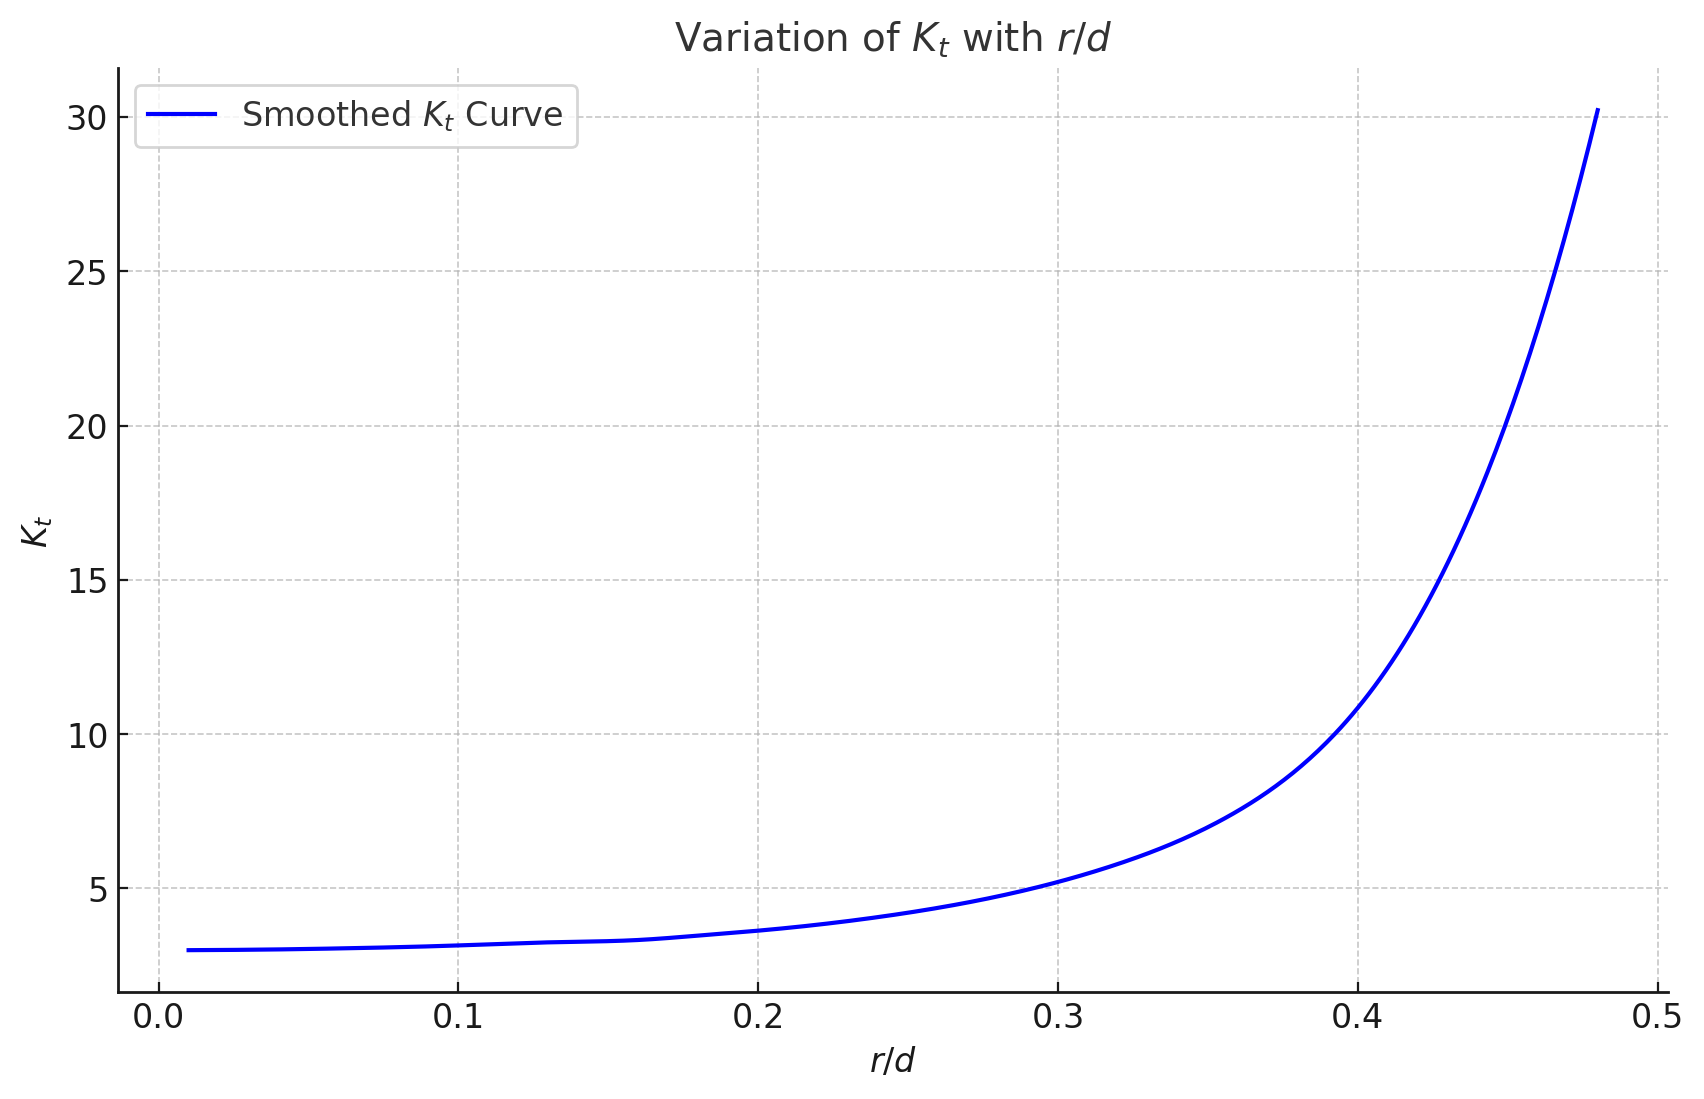
\includegraphics[width=\textwidth]{Variation of $K_t$ with $r:d$.png}
        \caption{Variation of \(K_t\) with \(r/d\)}
        \label{fig:Kt_vs_rd}
    \end{minipage}\hfill
    \begin{minipage}{0.45\textwidth}
        \centering
        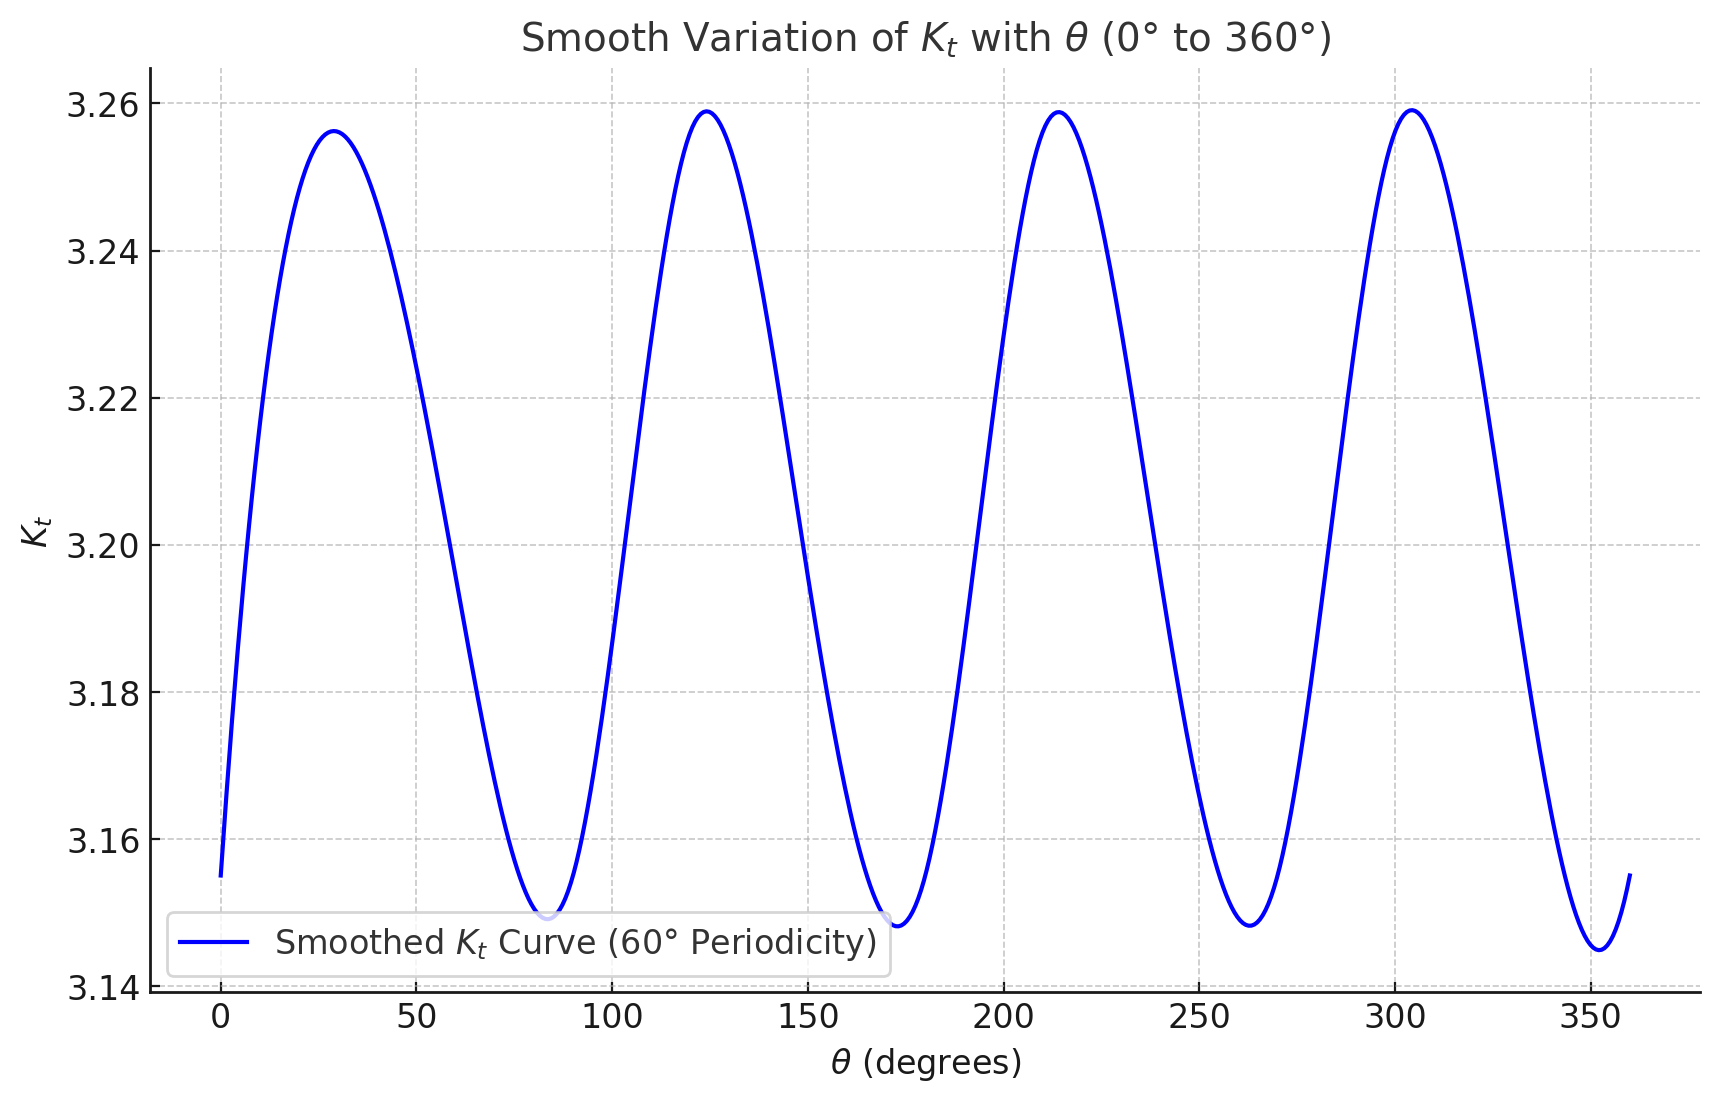
\includegraphics[width=\textwidth]{Smooth_Variation.png}
        \caption{Variation of \(K_t\) with \(\theta\) from 0° to 360°.}
        \label{fig:Kt_vs_theta}
    \end{minipage}
\end{figure}


\FloatBarrier % Forces figure to be placed before continuing
 
\subsection{Variation of Kt with r/d}
\vspace{-10pt}
The relationship between stress concentration factor ($K_t$) and hole spacing ratio ($r/d$) demonstrates three distinct behavioral regions, as illustrated in Figure \ref{fig:Kt_vs_rd} . For $r/d$ ratios below 0.2, $K_t$ maintains a relatively stable value around 3.0, indicating minimal stress field interaction between holes. As $r/d$ increases from 0.2 to 0.35, a moderate increase in $K_t$ is observed, suggesting the onset of stress field interference. Beyond $r/d = 0.35$, the curve exhibits exponential growth, with $K_t$ reaching approximately 30 at $r/d = 0.5$, indicating severe stress amplification.  The dramatic increase in $K_t$ at higher spacing ratios has significant implications for aircraft fuselage design, where multiple holes are required for riveted joints and system installations. For instance, in the design of an aircraft's pressure bulkhead, where holes are needed for hydraulic and electrical system pass-throughs\cite{cranfield_resource}, maintaining an $r/d$ ratio below 0.2 is crucial. At this ratio, the $K_t$ value remains around 3.0, providing a manageable stress concentration level. However, if space constraints force designers to place holes closer together, approaching an $r/d$ ratio of 0.4, the $K_t$ value could exceed 10, potentially leading to premature fatigue failure under cyclic pressurization loads. This phenomenon was notably observed in the de Havilland Comet accidents \cite{faa_galyv} of the 1950s, where closely spaced window corners led to catastrophic failures. Modern aerospace design practices now strictly regulate hole spacing, typically mandating minimum edge distances \cite{rivet_edge_distance} of 2D+0.05 times the hole diameter ($r/d \leq 0.2$)  throughout the aircraft's service life.

\vspace{-10pt}
\subsection{Variation of Kt with ($\theta$) }
\vspace{-10pt}

The variation of $K_t$ with load angle ($\theta$) shown in Figure \ref{fig:Kt_vs_theta}  exhibits a distinct periodic pattern, reflecting the threefold symmetry of the hole arrangement. Peak $K_t$ values of 3.258 occur at $\theta = 30^\circ$, $90^\circ$, $150^\circ$, $210^\circ$, $270^\circ$, and $330^\circ$, while minimum $K_t$ values of 3.147 are observed at $\theta = 0^\circ$, $60^\circ$, $120^\circ$, $180^\circ$, $240^\circ$, and $300^\circ$. The amplitude of variation ($\Delta K_t \approx 0.111$) remains consistent across all periods. This smooth sinusoidal variation suggests that the stress concentration factor behaves predictably under rotating loads, with the periodicity directly linked to the symmetry of the hole configuration. Such findings are essential for determining optimal loading orientations in real-world applications, where load angles may vary due to operational conditions. The smooth sinusoidal variation of $K_t$ with loading angle has direct implications for rotating machinery design, particularly in turbine disk applications. For example, in gas turbine engines, where multiple bolt holes secure the turbine disk to the shaft, understanding the angular dependence of stress concentration is crucial\cite{norton2019machine}. By aligning the holes \cite{meguid1995finite} with angles corresponding to minimum $K_t$ values, designers can reduce peak stresses during operation. This optimization becomes particularly significant during transient conditions, such as startup and shutdown\cite{rao2011mechanical}, where varying thermal and mechanical loads create complex stress states ,  utilised by major manufacturers like Rolls-Royce and GE Aviation. 

  

 


 \begin{figure}[h!]
 \subsection{Stress Concentration Factor with Reduced Plate Size}

    \centering
    \begin{minipage}{0.48\textwidth}
        \centering
        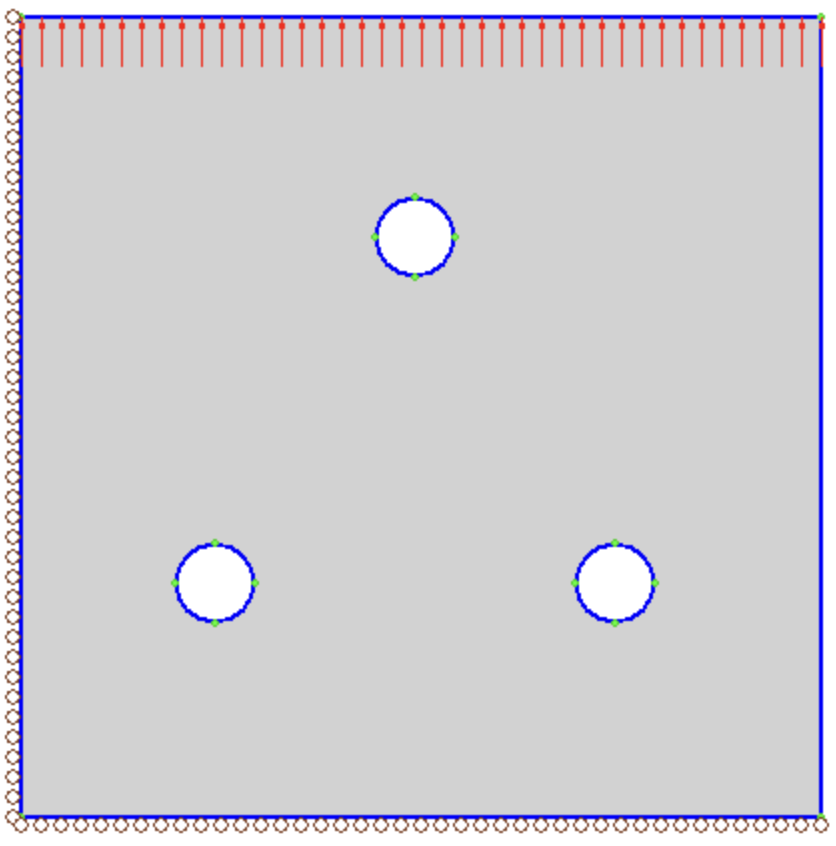
\includegraphics[height=6cm, keepaspectratio]{simulation model.png} % Replace with the actual file name
        \caption{ plate with three holes arranged in an equilateral triangle (\(r/d = 0.5\), \(d = 100\), \(\theta = 0\)). }
        \label{fig:simulation_model}
    \end{minipage}
    \hfill
    \begin{minipage}{0.48\textwidth}
        \centering
        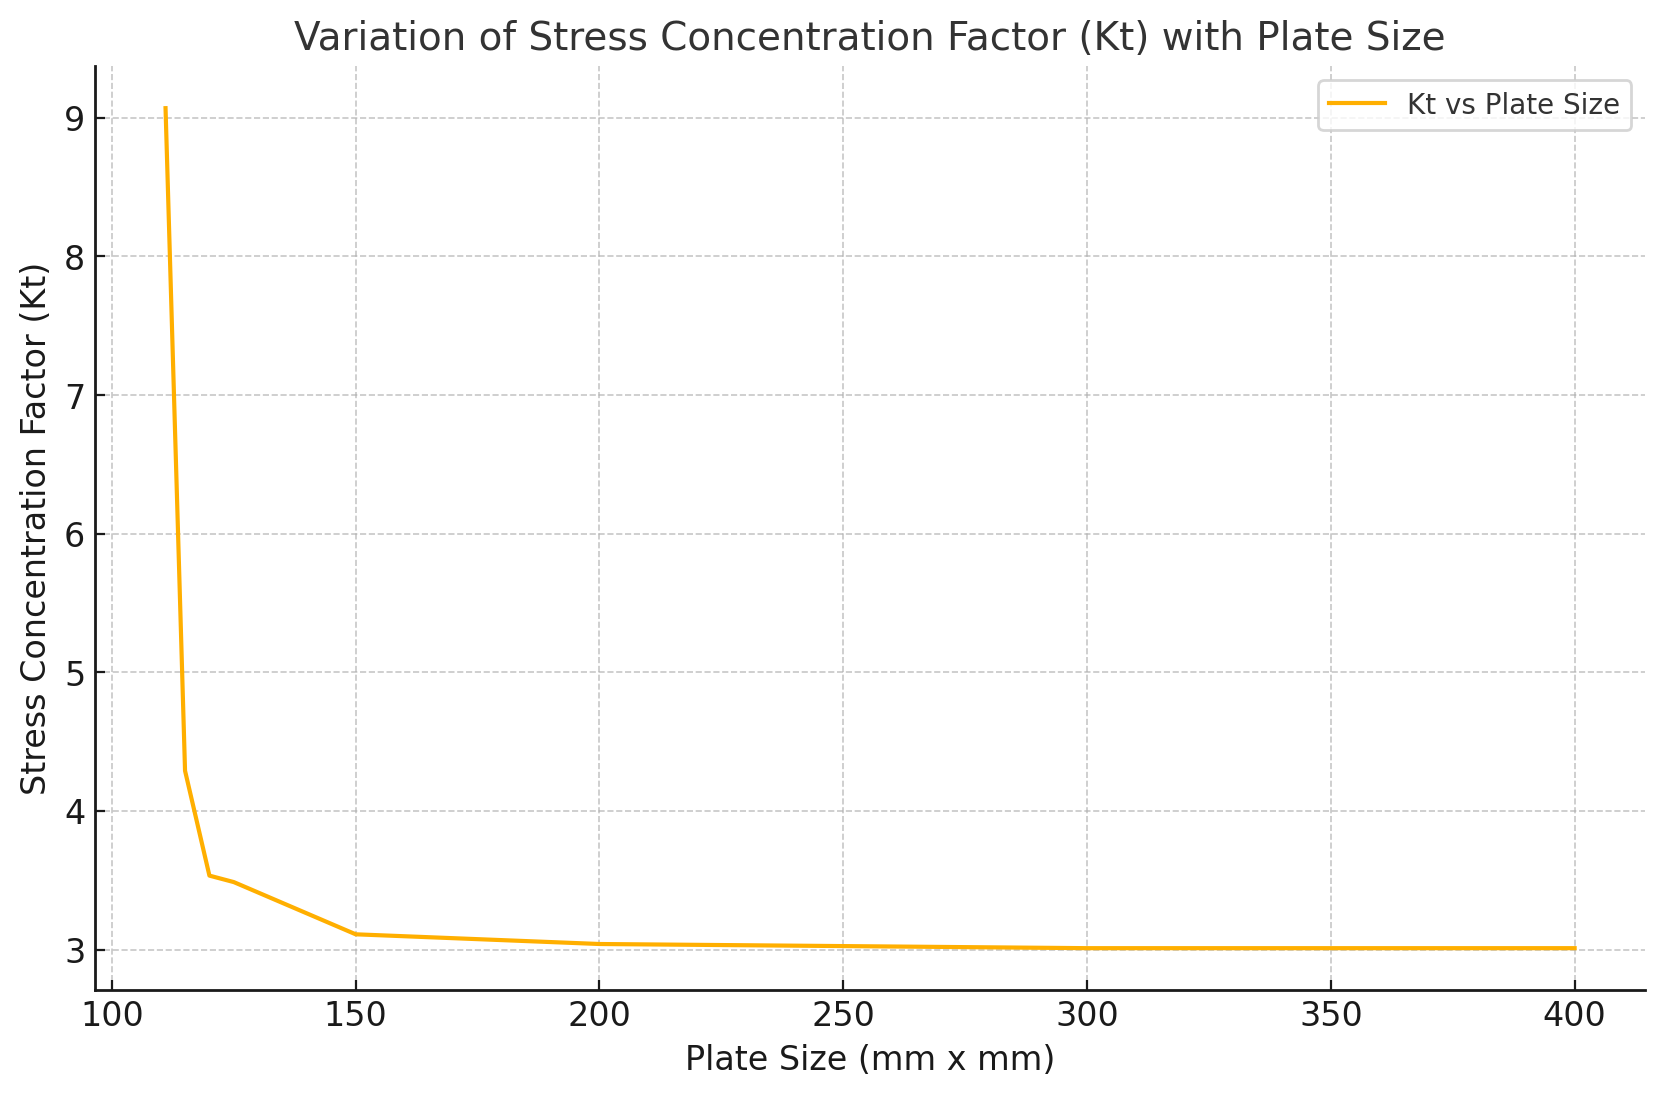
\includegraphics[height=6cm, keepaspectratio]{Variation of Stress Concentration Factor (Kt) with Plate Size.png} % Replace with the actual file name
        \caption{Variation of stress concentration factor (\(K_t\)) with plate size for the same configuration.}
        \label{fig:plate_size_effect}
    \end{minipage}
\end{figure}

  \FloatBarrier
The geometry of the holes and load direction (\(r/d\) and \(\theta\)) is fixed, and the plate size is progressively reduced. Reducing the plate width from \(400\, \mathrm{mm}\) to \(100 \, \mathrm{mm}\) increased \(K_t\) by 37\% for \(r/d = 0.1\) and \(\theta = 0^\circ\), emphasizing the influence of edge effects on stress concentration. These results are shown in Figure~\ref{fig:plate_size_effect}. The influence of plate size on the stress concentration factor ($K_t$) demonstrates a notable inverse relationship, as shown in Figure \ref{fig:plate_size_effect}. For smaller plate dimensions around 100mm $\times$ 100mm, $K_t$ exhibits a peak value of approximately 9.0, followed by a sharp decline. As the plate size increases to 150mm $\times$ 150mm, $K_t$ stabilizes around 3.0, after which further increases in plate dimensions have minimal impact on the stress concentration factor. This asymptotic behavior beyond 150mm $\times$ 150mm suggests that the stress field becomes effectively independent of plate size once a certain dimensional threshold is reached. The rapid decrease in $K_t$ at smaller plate sizes indicates a critical zone where the plate's boundaries significantly influence the stress distribution, while the plateau region at larger dimensions represents a more stable stress state where boundary effects become negligible. The relationship between plate size and stress concentration has significant implications in the design of aircraft wing panels, particularly in repair and modification scenarios. Consider a typical aluminum wing skin panel requiring a 25mm diameter inspection hole. If this hole is placed in a 100mm $\times$ 100mm repair patch, the high $K_t$ value (approximately 9.0) would necessitate additional reinforcement or alternative repair strategies. However, when the same hole is located in the original wing panel (typically 300mm $\times$ 300mm or larger), the $K_t$ value stabilizes around 3.0, representing a much more manageable stress state. This understanding has practical applications in aircraft maintenance procedures - for instance, Boeing's 737 repair manual \cite{boeing_737_overhaul} specifically requires inspection holes to be placed at least 150mm from any panel edge or existing discontinuity, ensuring operation in the stable $K_t$ region. Airlines like Lufthansa Technik \cite{lufthansa_predictive_maintenance} apply these principles during maintenance operations, where they must balance the need for access holes with structural integrity. 
\vspace{-10pt}
\section{Conclusion}
\vspace{-10pt}
This study of stress concentrations in aerospace structures revealed key findings for aircraft design optimization. Analysis of the A350-900 fuselage showed elliptical windows generate a stress concentration factor ($K_t$) of 2.72, with peak stresses of 247.42 MPa at $\beta = 0\degree$ and $180\degree$. For hole configurations, maintaining spacing ratios ($r/d \leq 0.2$) proved crucial, as stress amplification becomes exponential beyond $r/d = 0.35$. Computational validation through Concept Analyst confirmed theoretical predictions, demonstrating predictable $K_t$ variations with loading angle $\theta$. Material analysis showed CFRP and Ti-6Al-4V significantly outperform traditional aluminum alloys, achieving safety factors of 3.23 and 3.56 respectively, supporting the aerospace industry's shift toward hybrid CFRP-titanium solutions.
\vspace{-10pt}
\section{Recommendation for Future Work}
\vspace{-10pt}
The presence of multiple openings in aerospace structures introduces complex stress field interactions, which challenge traditional superposition principles. Future work should aim to refine the current findings through advanced methodologies, such as 3D finite element analysis (FEA), fatigue testing, and reinforcement evaluation. These techniques are critical for improving the safety, reliability, and cost-efficiency of aerospace designs.

Saint-Venant's Principle\cite{saintvenant} provides valuable insights into the localization of window-induced stress disturbances and serves as a foundation for optimizing window spacing and placement. While energy methods\cite{energy_methods} remain instrumental in analyzing fatigue, singular stress analysis\cite{sciencedirect2009} becomes less relevant due to the adoption of modern design practices, such as rounded window corners, which effectively mitigate sharp stress concentrations.

Advanced numerical methods like FEA are essential for accurately predicting stresses in complex geometries, accounting for three-dimensional effects such as through-thickness gradients and material anisotropy. Furthermore, the incorporation of von Mises failure criteria ensures structural integrity under cyclic pressurization loads, enhancing the reliability of critical components in aerospace structures.


 
 

\vspace{-10pt}
\bibliographystyle{unsrt}
\bibliography{references}
 
\vspace{-10pt}

\section{Appendix}
\vspace{-10pt}
Claude and Chatgpt is used to check syntax error and grammar mistakes.Cursor was used to improve the readability of matlab figure plotting code. And Chatgpt is used for formarting overleaf code, include formarting and hyperlinks.

 

\end{document}
